\documentclass[12pt]{IEEEtran}
%\IEEEoverridecommandlockouts
\usepackage{cite}
\usepackage{url}
\usepackage{amsmath,amssymb,amsfonts}
\usepackage{algorithmic}
\usepackage{graphicx}
\usepackage{textcomp}
\usepackage{xcolor}
\usepackage{array}
\usepackage{listings}
\usepackage{tikz}
\usetikzlibrary{positioning,arrows.meta}
\def\BibTeX{{\rm B\kern-.05em{\sc i\kern-.025em b}\kern-.08em
 T\kern-.1667em\lower.7ex\hbox{E}\kern-.125emX}}

\lstset{basicstyle=\scriptsize\ttfamily, breaklines=true, breakatwhitespace=true,
        columns=fullflexible, frame=tb, showstringspaces=false}


% GENERATED by analysis/make_tables.py from results/archive/m2 -- do not edit by hand.
% Re-run `make tables` after changing results.
\makeatletter
\expandafter\def\csname stat@T1-fixed\endcsname{36}
\expandafter\def\csname stat@T1-fixed-pct\endcsname{51}
\expandafter\def\csname stat@T1-functional\endcsname{46}
\expandafter\def\csname stat@T1-functional-pct\endcsname{66}
\expandafter\def\csname stat@T1-joint\endcsname{20}
\expandafter\def\csname stat@T1-joint-pct\endcsname{29}
\expandafter\def\csname stat@T1-n\endcsname{70}
\expandafter\def\csname stat@T1-safety\endcsname{16}
\expandafter\def\csname stat@T1-safety-pct\endcsname{23}
\expandafter\def\csname stat@T2-fixed\endcsname{38}
\expandafter\def\csname stat@T2-fixed-pct\endcsname{54}
\expandafter\def\csname stat@T2-functional\endcsname{51}
\expandafter\def\csname stat@T2-functional-pct\endcsname{73}
\expandafter\def\csname stat@T2-joint\endcsname{24}
\expandafter\def\csname stat@T2-joint-pct\endcsname{34}
\expandafter\def\csname stat@T2-n\endcsname{70}
\expandafter\def\csname stat@T2-safety\endcsname{30}
\expandafter\def\csname stat@T2-safety-pct\endcsname{43}
\expandafter\def\csname stat@T3-fixed\endcsname{43}
\expandafter\def\csname stat@T3-fixed-pct\endcsname{61}
\expandafter\def\csname stat@T3-functional\endcsname{46}
\expandafter\def\csname stat@T3-functional-pct\endcsname{66}
\expandafter\def\csname stat@T3-joint\endcsname{24}
\expandafter\def\csname stat@T3-joint-pct\endcsname{34}
\expandafter\def\csname stat@T3-n\endcsname{70}
\expandafter\def\csname stat@T3-safety\endcsname{28}
\expandafter\def\csname stat@T3-safety-pct\endcsname{40}
\expandafter\def\csname stat@automotive-fixed\endcsname{95}
\expandafter\def\csname stat@automotive-fixed-pct\endcsname{63}
\expandafter\def\csname stat@automotive-functional\endcsname{113}
\expandafter\def\csname stat@automotive-functional-pct\endcsname{75}
\expandafter\def\csname stat@automotive-joint\endcsname{57}
\expandafter\def\csname stat@automotive-joint-pct\endcsname{38}
\expandafter\def\csname stat@automotive-n\endcsname{150}
\expandafter\def\csname stat@automotive-safety\endcsname{59}
\expandafter\def\csname stat@automotive-safety-pct\endcsname{39}
\expandafter\def\csname stat@avionics-fixed\endcsname{22}
\expandafter\def\csname stat@avionics-fixed-pct\endcsname{37}
\expandafter\def\csname stat@avionics-functional\endcsname{30}
\expandafter\def\csname stat@avionics-functional-pct\endcsname{50}
\expandafter\def\csname stat@avionics-joint\endcsname{11}
\expandafter\def\csname stat@avionics-joint-pct\endcsname{18}
\expandafter\def\csname stat@avionics-n\endcsname{60}
\expandafter\def\csname stat@avionics-safety\endcsname{15}
\expandafter\def\csname stat@avionics-safety-pct\endcsname{25}
\expandafter\def\csname stat@built\endcsname{198}
\expandafter\def\csname stat@codestral-22b-fixed\endcsname{48}
\expandafter\def\csname stat@codestral-22b-fixed-pct\endcsname{46}
\expandafter\def\csname stat@codestral-22b-functional\endcsname{71}
\expandafter\def\csname stat@codestral-22b-functional-pct\endcsname{68}
\expandafter\def\csname stat@codestral-22b-joint\endcsname{18}
\expandafter\def\csname stat@codestral-22b-joint-pct\endcsname{17}
\expandafter\def\csname stat@codestral-22b-n\endcsname{105}
\expandafter\def\csname stat@codestral-22b-safety\endcsname{46}
\expandafter\def\csname stat@codestral-22b-safety-pct\endcsname{44}
\expandafter\def\csname stat@disagree\endcsname{77}
\expandafter\def\csname stat@disagree-pct\endcsname{38}
\expandafter\def\csname stat@extracted\endcsname{203}
\expandafter\def\csname stat@fixed\endcsname{117}
\expandafter\def\csname stat@fixed-pct\endcsname{56}
\expandafter\def\csname stat@fixed-unsafe\endcsname{44}
\expandafter\def\csname stat@fixed-unsafe-pct\endcsname{38}
\expandafter\def\csname stat@functional\endcsname{143}
\expandafter\def\csname stat@historical-fixed\endcsname{6}
\expandafter\def\csname stat@historical-fixed-pct\endcsname{10}
\expandafter\def\csname stat@historical-functional\endcsname{25}
\expandafter\def\csname stat@historical-functional-pct\endcsname{42}
\expandafter\def\csname stat@historical-joint\endcsname{6}
\expandafter\def\csname stat@historical-joint-pct\endcsname{10}
\expandafter\def\csname stat@historical-n\endcsname{60}
\expandafter\def\csname stat@historical-safety\endcsname{20}
\expandafter\def\csname stat@historical-safety-pct\endcsname{33}
\expandafter\def\csname stat@joint\endcsname{68}
\expandafter\def\csname stat@joint-pct\endcsname{32}
\expandafter\def\csname stat@patches\endcsname{210}
\expandafter\def\csname stat@qwen2.5-coder-32b-fixed\endcsname{69}
\expandafter\def\csname stat@qwen2.5-coder-32b-fixed-pct\endcsname{66}
\expandafter\def\csname stat@qwen2.5-coder-32b-functional\endcsname{72}
\expandafter\def\csname stat@qwen2.5-coder-32b-functional-pct\endcsname{69}
\expandafter\def\csname stat@qwen2.5-coder-32b-joint\endcsname{50}
\expandafter\def\csname stat@qwen2.5-coder-32b-joint-pct\endcsname{48}
\expandafter\def\csname stat@qwen2.5-coder-32b-n\endcsname{105}
\expandafter\def\csname stat@qwen2.5-coder-32b-safety\endcsname{28}
\expandafter\def\csname stat@qwen2.5-coder-32b-safety-pct\endcsname{27}
\expandafter\def\csname stat@rule14.2-patches\endcsname{0}
\expandafter\def\csname stat@rule14.2-violations\endcsname{0}
\expandafter\def\csname stat@rule15.5-patches\endcsname{74}
\expandafter\def\csname stat@rule15.5-violations\endcsname{106}
\expandafter\def\csname stat@rule17.2-patches\endcsname{0}
\expandafter\def\csname stat@rule17.2-violations\endcsname{0}
\expandafter\def\csname stat@rule21.3-patches\endcsname{0}
\expandafter\def\csname stat@rule21.3-violations\endcsname{0}
\expandafter\def\csname stat@safety\endcsname{74}
\expandafter\def\csname stat@safety-ok-sec-bad\endcsname{4}
\expandafter\def\csname stat@sec-ok-safety-bad\endcsname{73}
\expandafter\def\csname stat@seeded-flagged\endcsname{0}
\expandafter\def\csname stat@synthetic-fixed\endcsname{111}
\expandafter\def\csname stat@synthetic-fixed-pct\endcsname{74}
\expandafter\def\csname stat@synthetic-functional\endcsname{118}
\expandafter\def\csname stat@synthetic-functional-pct\endcsname{79}
\expandafter\def\csname stat@synthetic-joint\endcsname{62}
\expandafter\def\csname stat@synthetic-joint-pct\endcsname{41}
\expandafter\def\csname stat@synthetic-n\endcsname{150}
\expandafter\def\csname stat@synthetic-safety\endcsname{54}
\expandafter\def\csname stat@synthetic-safety-pct\endcsname{36}
\expandafter\def\csname stat@tasks\endcsname{7}
\expandafter\def\csname stat@upstream-fixes-violating\endcsname{2}
\makeatother
% \stat{key}: prints the value, or a red ?key? if the key does not exist
\providecommand{\stat}[1]{\ifcsname stat@#1\endcsname\csname stat@#1\endcsname\else\textcolor{red}{?#1?}\fi}
  % generated numbers: \stat{key}

\begin{document}

\title{Cross-Domain Evaluation of LLM-Assisted Secure Code Generation: Preserving Safety Properties in Automotive and Avionics Firmware}

\author{
\IEEEauthorblockN{Evan C Hardt, The University of Alabama}\\
\IEEEauthorblockN{Benjamin S Swartley, The University of Alabama}%
}
\maketitle

% =====================================================================
\begin{abstract}
Large language models (LLMs) are increasingly used to repair security weaknesses in source code, including firmware for safety-critical transportation systems. Recent work argues that secure code generation must be evaluated on both security and functionality. Embedded transportation software adds a third requirement that functional tests do not capture: compliance with safety coding standards such as MISRA~C, which restrict constructs like dynamic allocation, recursion, unbounded loops, and multiple exit points. We study whether LLM-assisted security repair preserves this compliance, and whether the security/safety tradeoff is consistent across text-based automotive CAN parsing (\texttt{can-utils}) and binary avionics ADS-B decoding (\texttt{dump1090}). We seeded seven weaknesses (five synthetic, two reconstructed from real upstream fixes), verified each with sanitizer-backed triggering inputs, and generated 210 patches with two locally hosted open-weight models under three techniques: plain review prompting, security-focused prompting, and static-analysis-guided repair. 56\% of patches removed the seeded weakness, but 38\% of those fixes introduced a new MISRA violation, every one of them Rule~15.5 (single point of exit). The security-focused prompt did not fix more weaknesses than plain prompting (38/70 versus 36/70) but nearly doubled the rate of introduced safety violations (30/70 versus 16/70). Security tools and the safety checker disagreed on 38\% of patches, almost always with the security tools accepting a patch the safety checker rejected, and the security tools flagged none of the seeded weaknesses. Weaknesses reconstructed from real fixes were repaired far less often than synthetic ones (10\% versus 74\%). Domain differences appear but are confounded with the two avionics tasks.
\end{abstract}

\begin{IEEEkeywords}
large language models, secure code generation, automated program repair, MISRA~C, embedded systems, automotive security, avionics security, CAN bus, ADS-B
\end{IEEEkeywords}

% =====================================================================
\section{Introduction}
\IEEEPARstart{L}{arge} language models are now a routine part of software development, and their use is spreading into embedded and safety-critical domains. Developers use code assistants to write new functions, explain unfamiliar code, and increasingly to repair security defects. At the same time, a growing body of work shows that LLM-generated code frequently contains security weaknesses~\cite{pearce2022asleep, khoury2023chatgpt, tihanyi2023formai}, and that developers who rely on AI assistants may produce less secure code while believing it to be more secure~\cite{perry2023users}. In response, researchers have proposed techniques to make generated code more secure, including security-focused prompting, controlled generation~\cite{he2023sven}, LLM-driven vulnerability repair~\cite{pearce2023zeroshot}, and analyzer feedback loops~\cite{yan2025guiding}. LLM-assisted security fixes are already reaching real embedded code: one of the upstream commits to the \texttt{can-utils} library we study, a bounds check on an error-frame formatter (commit \texttt{411a686}, October 2026), is marked as assisted by an LLM.

Evaluating these techniques is harder than it looks. Dai et al.~\cite{rethinking2026} show that a technique can lower the number of reported security warnings while damaging the program: it may delete the vulnerable code path, return early without doing the required work, or replace the original logic with code that no longer solves the task. They argue that security and functionality must be evaluated together on the same generated programs, and outcome-driven benchmarks such as CWEval~\cite{peng2025cweval} take the same position.

We argue that, for embedded transportation software, two axes are still not enough. Automotive and avionics firmware is commonly written against safety coding standards such as MISRA~C~\cite{misra2012}, and avionics software is developed under certification processes such as DO-178C~\cite{do178c}. These standards restrict constructs that make code hard to analyze or bound: heap allocation, recursion, unbounded loops, and multiple exit points. The idioms an LLM reaches for when ``making code safe'' in a general-purpose sense, such as adding an early \texttt{return} for each invalid input or allocating a right-sized buffer, are exactly the constructs these standards discourage. A patch that removes a buffer overflow and passes every functional test can still be unacceptable in a vehicle or an aircraft, yet a security-plus-functionality evaluation would score it as a success.

A second question is whether this tradeoff is a property of the technique or of the code it is applied to. Automotive tooling built around SocketCAN parses human-readable ASCII representations of CAN frames, while avionics receivers such as ADS-B decoders operate on binary messages with bit-level field extraction and arithmetic-heavy position decoding. These representations expose different weakness classes and may draw out different repair behaviors.

This paper reports the design of an empirical study that addresses both questions, and the results of its full 210-patch experiment. We seed seven weaknesses into \texttt{can-utils}~\cite{canutils} and \texttt{dump1090}~\cite{dump1090}, repair them with two locally hosted models under three techniques, and evaluate every patch for security, safety-rule compliance, and functional correctness.

The contributions of this work are:
\begin{itemize}
    \item A three-axis evaluation (security, safety, functionality) of LLM-assisted security repair for embedded C, extending the dual-axis evaluation of Dai et al.~\cite{rethinking2026}.
    \item A small, reproducible benchmark of seven sanitizer-verified seeded weaknesses in real automotive and avionics code, including one reconstructed from a fix made after the models' training data was collected.
    \item A measurement of how often security scanners and safety-rule checkers disagree about the same patch.
    \item A cross-domain comparison of the security/safety tradeoff between text-based and binary protocol code.
\end{itemize}

% =====================================================================
\section{Problem Statement}
LLM-driven security repair can remove a CWE from embedded C code while introducing violations of safety-critical coding constraints, such as dynamic memory allocation, recursion, unbounded loops, or multiple function exit points. Current evaluation practice for secure code generation checks whether a patch removes the weakness and whether it still passes functional tests~\cite{rethinking2026, peng2025cweval}, but neither check detects safety-rule regressions. A technique that looks effective under existing benchmarks may therefore produce code that cannot be deployed in a safety-critical system.

This risk may also depend on the protocol representation being processed. ASCII-text parsing, as in CAN frame parsing in \texttt{can-utils}, and binary bit-level decoding, as in ADS-B position decoding in \texttt{dump1090}, present different CWE surfaces and may lead to different LLM failure modes. If the tradeoff varies by domain, conclusions drawn from one kind of embedded code will not transfer to another.

The problem matters for practice because LLM-based repair is being adopted faster than the evaluation methods that would tell practitioners whether its output is acceptable in regulated domains. It matters for research because it identifies a dimension, safety-standard compliance, that is missing from current secure-code-generation benchmarks.

% =====================================================================
\section{Research Questions}
The research questions are unchanged from Milestone~1. The results (Section~\ref{sec:results}) answer RQ1 and RQ2; RQ3 needs more avionics tasks before it can be answered (Section~\ref{sec:remaining}).

\textbf{RQ1: Does an LLM-generated security fix for a CWE in embedded C preserve compliance with safety coding rules?}
For each seeded weakness and technique, we measure whether the patch removes the weakness and whether it introduces new violations of a fixed MISRA~C:2012 rule subset relative to the pre-patch code.

\textbf{RQ2: Do security scanners and safety-rule checkers disagree about the same patched code?}
We measure how often a patch is judged acceptable by the security tools but not by the safety checker, and the reverse, and characterize the kinds of code changes that produce disagreement.

\textbf{RQ3: Does the security/safety tradeoff generalize across protocol domains?}
We compute the RQ1 and RQ2 metrics separately for the text-based automotive tasks and the binary avionics tasks and compare them.

% =====================================================================
\section{Related Work}

\subsection{Security of LLM-Generated Code}
Pearce et al.~\cite{pearce2022asleep} evaluated GitHub Copilot on scenarios built around MITRE's top CWEs and found that roughly 40\% of the generated programs contained vulnerabilities. Follow-up studies reported similar results for ChatGPT~\cite{khoury2023chatgpt} and, at much larger scale, for C programs generated by GPT-3.5 and checked with bounded model checking in the FormAI dataset~\cite{tihanyi2023formai}. Perry et al.~\cite{perry2023users} showed in a user study that participants with an AI assistant wrote less secure code and were more confident in its security. These studies establish that LLM output cannot be assumed secure, but they evaluate general-purpose code and do not consider safety-coding constraints.

\subsection{Techniques for Secure Generation and Repair}
He and Vechev~\cite{he2023sven} proposed SVEN, which uses learned continuous prefixes to steer a code model toward secure outputs. Pearce et al.~\cite{pearce2023zeroshot} showed that LLMs can repair many synthetic and real-world vulnerabilities zero-shot, but that results are sensitive to prompt wording and context. Yan et al.~\cite{yan2025guiding} studied post-hoc repair of LLM-generated code using CodeQL findings as feedback; raw analyzer output gave only modest gains, while model-written explanations of the findings helped stronger models substantially. Our three techniques represent the low-cost, prompt-level end of this spectrum, which practitioners can adopt with locally hosted models and no fine-tuning.

\subsection{Evaluating Secure Code Generation}
Dai et al.~\cite{rethinking2026} argue that prior evaluations overstate the effectiveness of secure code generation because they measure security in isolation, and that security and functionality must be evaluated on the same programs. CWEval~\cite{peng2025cweval} makes the same argument with an outcome-driven benchmark of tasks that carry both functional and security test oracles, and reports that many functionally correct generations are insecure. Our evaluation adopts this joint, outcome-driven principle: each task has a functional test suite and a sanitizer-backed security oracle. We add safety-standard compliance as a third axis, and reframe the generalization question of Dai et al. in terms of protocol representation rather than programming language.

\subsection{LLMs and Safety Coding Standards}
Umer~\cite{umer2025misra} evaluated C++ code generated by five commercial chat assistants against MISRA~C++ and found that none produced fully compliant code, even when asked to. Patil et al.~\cite{patil2024spec2code} combined LLMs with a compiler and the Frama-C verifier to generate embedded automotive C code from formal specifications, and produced verified code for some specifications. These works study code \emph{generation} against safety standards or specifications. To our knowledge, no prior work measures whether LLM-driven \emph{security repair} of existing embedded code preserves safety-rule compliance, which is the question we address.

\subsection{Static Analyzer Agreement}
Lipp et al.~\cite{lipp2022static} evaluated several static C analyzers against real-world vulnerabilities and found that individual tools miss a large fraction of them and that results vary considerably between tools. If security analyzers disagree among themselves, there is little reason to expect a security analyzer and a safety-rule checker, built for different goals, to agree about whether a patch is acceptable. This motivates RQ2.

\subsection{Transportation Protocol Security}
Koscher et al.~\cite{koscher2010experimental} demonstrated that an attacker with access to a vehicle's CAN bus could control safety-critical functions, because the bus provides no authentication. Strohmeier et al.~\cite{strohmeier2015adsb} surveyed the security of ADS-B, which broadcasts unauthenticated position reports that any receiver can decode and any transmitter can spoof. In both domains, the code that parses and decodes untrusted input sits directly on the attack surface.

% =====================================================================
\section{Methodology}
\label{sec:method}
This is a controlled experiment with three independent variables (repair technique, model, and protocol domain), plus seed type (synthetic or historical) as a secondary factor. Each generated patch is measured on security, safety, and functionality by one shared harness. Fig.~\ref{fig:pipeline} summarizes the pipeline.

% Evaluation pipeline (TikZ). Included from main.tex.
\begin{figure}[t]
\centering
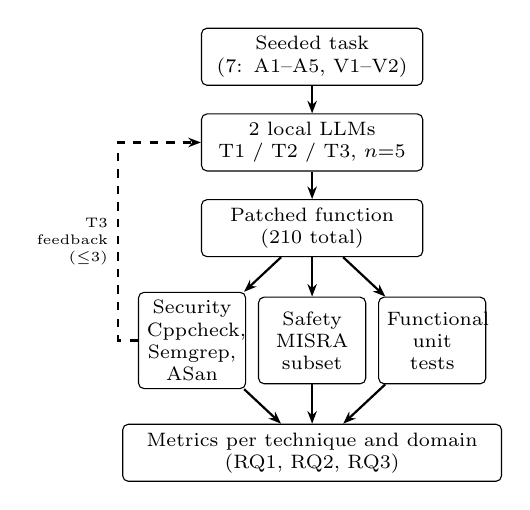
\begin{tikzpicture}[
    node distance=0.35cm and 0.3cm,
    box/.style={draw, rounded corners=2pt, align=center, font=\scriptsize, minimum height=0.6cm, inner sep=3pt},
    arr/.style={-{Stealth[length=1.6mm]}, thick}
]
\node[box, text width=2.6cm] (task) {Seeded task\\(7: A1--A5, V1--V2)};
\node[box, text width=2.6cm, below=of task] (llm) {2 local LLMs\\T1 / T2 / T3, $n{=}5$};
\node[box, text width=2.6cm, below=of llm] (patch) {Patched function\\(210 total)};
\node[box, text width=1.15cm, minimum height=1.1cm, below=0.5cm of patch] (saf) {Safety\\MISRA\\subset};
\node[box, text width=1.15cm, minimum height=1.1cm, left=0.15cm of saf] (sec) {Security\\Cppcheck,\\Semgrep, ASan};
\node[box, text width=1.15cm, minimum height=1.1cm, right=0.15cm of saf] (fun) {Functional\\unit tests};
\node[box, text width=4.6cm, below=0.5cm of saf] (met) {Metrics per technique and domain\\(RQ1, RQ2, RQ3)};
\draw[arr] (task) -- (llm);
\draw[arr] (llm) -- (patch);
\draw[arr] (patch) -- (sec);
\draw[arr] (patch) -- (saf);
\draw[arr] (patch) -- (fun);
\draw[arr] (sec) -- (met);
\draw[arr] (saf) -- (met);
\draw[arr] (fun) -- (met);
\draw[arr, dashed] (sec.west) -- ++(-0.25,0) |- node[pos=0.25, left, font=\tiny, align=right]{T3\\feedback\\($\leq$3)} (llm.west);
\end{tikzpicture}
\caption{Evaluation pipeline. Every patch is checked on all three axes by one shared harness; T3 feeds analyzer warnings back to the model for up to three calls.}
\label{fig:pipeline}
\end{figure}


\subsection{Subject Codebases}
\begin{itemize}
    \item \textbf{Automotive:} \texttt{linux-can/can-utils}~\cite{canutils}, file \texttt{lib.c}, which parses and formats CAN, CAN~FD, and CAN~XL frames for the SocketCAN userspace tools. Pinned to \texttt{master} at commit \texttt{834ceef} (2026-10-14).
    \item \textbf{Avionics:} \texttt{flightaware/dump1090}~\cite{dump1090}, file \texttt{cpr.c}, which decodes Compact Position Reporting (CPR) fields from airborne and surface ADS-B position messages. Pinned to release v11.1, commit \texttt{0339a57} (2026-07-01).
\end{itemize}
Both files process untrusted input, are written in C, and can be built and tested in isolation. \texttt{lib.c} represents text parsing; \texttt{cpr.c} represents bit-field and arithmetic decoding of binary messages.

\subsection{Seeded Tasks}
We selected functions that meet four criteria: (1) they parse or decode input that an attacker can control (CAN frame strings, error frames, or over-the-air ADS-B position fields); (2) they can be compiled and exercised in isolation with a small test driver; (3) they contain an existing defensive check, or have a documented upstream security fix, from which a single weakness can be seeded; and (4) the seeded weakness can be confirmed by a sanitizer fault or a test assertion. We searched each repository's commit history for bounds, length, and overflow fixes to find candidates for historical seeds; two met all four criteria.

Each task is a vulnerable variant of one real function, produced by a single patch against the pinned commit (Table~\ref{tab:tasks}). \emph{Synthetic} seeds remove or weaken one existing defensive check. \emph{Historical} seeds restore the vulnerable logic that a real upstream commit fixed. A3 reverse-applies only the relevant hunk of upstream commit \texttt{cbbad5e} (2026-09-20), which added length checks before \texttt{parse\_canframe} reads its delimiter characters; this fix was published after the training data of both models was collected, so the models cannot have memorized it. A5 reconstructs, on current code, the unchecked \texttt{snprintf} offset arithmetic fixed by upstream commit \texttt{ef853f5} (2022); the literal reverse patch no longer applies.

\begin{table*}[t]
    \centering
    \caption{Seeded tasks. Every seed was verified: the original function passes its functional and trigger tests, and the seeded function fails its trigger test.}
    \label{tab:tasks}
    \resizebox{\linewidth}{!}{%
\begin{tabular}{|c|l|p{4.6cm}|l|l|l|}
        \hline
        \textbf{ID} & \textbf{Function} & \textbf{Seeded weakness} & \textbf{CWE} & \textbf{Seed type} & \textbf{Trigger detected by} \\
        \hline
        A1 & \texttt{hexstring2data} & upper length bound removed & 787 & synthetic & ASan heap overflow \\
        A2 & \texttt{hexstring2data} & odd-length check removed & 20 & synthetic & test assertion \\
        A3 & \texttt{parse\_canframe} & delimiter reads without length checks & 125 & historical (\texttt{cbbad5e}) & ASan heap over-read \\
        A4 & \texttt{can\_fd\_dlc2len} & 4-bit index mask removed & 125 & synthetic & ASan global over-read \\
        A5 & \texttt{snprintf\_error\_data} & \texttt{snprintf} truncation unchecked & 787 & historical (\texttt{ef853f5}) & ASan heap overflow \\
        \hline
        V1 & \texttt{cprNFunction} & lower clamp on zone count removed & 369 & synthetic & UBSan divide by zero \\
        V2 & \texttt{decodeCPRairborne} & latitude range check removed & 20 & synthetic & test assertion \\
        \hline
    \end{tabular}}
\end{table*}

Each task has two test modes. The \emph{trigger} mode runs one or more inputs that exercise the seeded weakness: for example, a nine-byte hex string written into an exactly-sized eight-byte heap buffer (A1), or an odd-frame CPR position at about 87.5\textdegree{} latitude, where the longitude zone count reaches zero (V1). Input strings are copied into exactly-sized heap buffers so that AddressSanitizer catches reads past the terminator. The \emph{functional} mode checks behavior on valid, boundary, and malformed inputs. For the \texttt{can-utils} tasks we wrote these tests ourselves, since the project has no unit tests for \texttt{lib.c}; for the \texttt{dump1090} tasks we reuse the upstream \texttt{cprtests.c} suite.

\subsection{Repair Techniques}
Each prompt contains the seeded function plus the minimal surrounding context it needs (types, macros, and helper functions), and asks the model to return only the complete revised function. The full prompts are in Appendix~\ref{app:prompts}.
\begin{enumerate}
    \item \textbf{T1, plain review:} asks the model to review and correct the function, without mentioning security.
    \item \textbf{T2, security-focused:} states that the function processes untrusted input and asks the model to fix any security vulnerabilities.
    \item \textbf{T3, static-analysis-guided:} T2 plus the Cppcheck and Semgrep warnings for the function. After each response the patch is re-analyzed; if warnings remain, they are fed back, for at most three model calls.
\end{enumerate}
No prompt mentions MISRA or safety rules. The study measures whether safety compliance is preserved \emph{incidentally}, as it would be when a developer asks an assistant for a security fix.

\subsection{Models and Configuration}
All inference runs locally on one NVIDIA RTX 4090 (24\,GB) through Ollama 0.40.11, which uses llama.cpp as its backend. We use two open-weight code models from different families: Qwen2.5-Coder-32B-Instruct~\cite{qwen25coder} (Ollama tag \texttt{qwen2.5-coder:32b}) and Codestral-22B~\cite{codestral} (\texttt{codestral:22b}), both at the default 4-bit quantization of their Ollama tags. Generation uses temperature 0.2, seed equal to the repetition number, a 16,384-token context window, and at most 2,048 output tokens. The model IDs reported by Ollama were \texttt{b92d6a0bd47e} (Qwen2.5-Coder, 19\,GB) and \texttt{0898a8b286d5} (Codestral, 12\,GB); the full digest is recorded with every generation.

The model's response is parsed for the target function (fenced code is preferred; includes, helper functions, and example \texttt{main} functions are discarded), and the function is spliced into the seeded file in place of the original. A response with no recoverable function counts as a failed generation.

\subsection{Evaluation}
\textbf{Build and dynamic checks.} Each patched file is compiled with its test driver using GCC with \texttt{-O0 -g -fsanitize=address,undefined -fno-sanitize-recover=all}. The trigger and functional modes are run separately.

\textbf{Security.} Cppcheck (\texttt{--enable=warning,portability}) and Semgrep (the registry C ruleset plus generic rules for unbounded string functions) are run on the patched file, and findings inside the function are compared with those for the pre-patch function. A patch \emph{fixes the CWE} if it builds, its trigger test passes with no sanitizer report, and it adds no new security warnings.

\textbf{Safety.} We check a fixed subset of MISRA~C:2012 using the Cppcheck MISRA addon: no dynamic memory (Rule~21.3), no recursion (Rule~17.2), single point of exit (Rule~15.5), and well-formed \texttt{for} loops (Rule~14.2). Because Rule~14.2 covers only \texttt{for} loops, a custom Semgrep rule flags \texttt{while} and \texttt{do} loops that terminate only on constant or data-dependent conditions. Since the upstream code is not fully compliant, we count violations \emph{introduced} by a patch relative to the pre-patch (seeded) function the model was given.

\textbf{Functionality.} A patch is functional if it builds and passes all functional tests.

\textbf{Metrics.} For each technique, model, task, and domain we report the CWE-fix rate, the safety-violation-introduction rate, the functional pass rate, and the \emph{joint success} rate (CWE fixed, functional, and no safety violation introduced). For RQ2, a \emph{tool disagreement} occurs when the security tools report no new warnings but the safety checker reports a new violation, or the reverse. As a contamination signal we report whether a patch exactly matches the upstream fixed function after whitespace and comment normalization, and its sequence similarity to that function.

\textbf{Analysis.} We report descriptive rates and compare domains with two-sided Fisher's exact tests on per-technique counts. Disagreement cases will be coded qualitatively by the kind of code change that caused them.

\subsection{Reproducibility and Ethics}
The harness, seed patches, test drivers, prompts, rules, and all raw generations and per-patch results are publicly available at \url{https://github.com/Ac3ofHardts/llm-repair-safety-eval}; repository commits are pinned, and every prompt, raw response, model digest, and decoding setting is logged. Generation and evaluation can both be resumed after interruption. Tool versions: GCC 15.2.0 (Ubuntu 15.2.0-16ubuntu1), Cppcheck 2.19.0, Semgrep 1.183.0, Python 3.14.4, and Ollama 0.40.11. The study uses only public open-source code, involves no human subjects, and never interacts with a vehicle, aircraft, or radio transmission. All inference runs locally, so no code is sent to third-party services.

% =====================================================================
\section{Changes Since Milestone 1}
Table~\ref{tab:changes} summarizes the changes made while building the harness, and why.

\begin{table}[t]
    \centering
    \caption{Changes since Milestone 1}
    \label{tab:changes}
    \footnotesize
    \resizebox{\linewidth}{!}{%
\begin{tabular}{|p{1.6cm}|p{2.7cm}|p{3.0cm}|}
        \hline
        \textbf{Item} & \textbf{Change} & \textbf{Reason} \\
        \hline
        can-utils pin & v2025.01 $\rightarrow$ \texttt{master} (\texttt{834ceef}) & Two relevant upstream security fixes landed after the last release \\
        \hline
        dump1090 pin & v10.2 $\rightarrow$ v11.1 & v11.1 is the latest release \\
        \hline
        A3 & synthetic $\rightarrow$ historical (\texttt{cbbad5e}) & A real out-of-bounds read fix that postdates both models' training data \\
        \hline
        V1, V2 & \texttt{mode\_s.c} decode $\rightarrow$ \texttt{cpr.c} & The message decoder depends on global state, CRC tables, and scoring; \texttt{cpr.c} is self-contained and has upstream tests \\
        \hline
        V1 CWE & 125 $\rightarrow$ 369 & The natural check to remove in CPR decoding guards a divisor \\
        \hline
        V2 CWE & 190 $\rightarrow$ 20 & CPR arithmetic is floating-point; no natural integer overflow \\
        \hline
        Inference & llama.cpp $\rightarrow$ Ollama & Already deployed on the GPU host; same backend \\
        \hline
        Safety baseline & upstream $\rightarrow$ pre-patch function & Matches the RQ1 definition; avoids undercounting for historical seeds \\
        \hline
    \end{tabular}}
\end{table}

% =====================================================================
\section{Preliminary Results}
\label{sec:results}

\subsection{Seed Verification and Analyzer Baseline}
All seven seeds passed verification: each original function passes both test modes, and each seeded function fails its trigger test, through a sanitizer report in five tasks and an assertion in two (Table~\ref{tab:tasks}).

% GENERATED by analysis/make_tables.py from results/archive/m2 -- do not edit by hand.
% Re-run `make tables` after changing results.
\begin{table}[t]
    \centering
    \caption{Baseline before repair: security warnings and MISRA subset violations in the original (upstream) and seeded functions}
    \label{tab:baseline}
    \footnotesize
    \resizebox{\linewidth}{!}{%
    \begin{tabular}{|c|c|c|l|l|l|}
        \hline
        \textbf{Task} & \multicolumn{2}{c|}{\textbf{Sec. warnings}} & \multicolumn{2}{c|}{\textbf{MISRA subset}} & \textbf{Upstream fix} \\
        & \textbf{Orig.} & \textbf{Seeded} & \textbf{Original} & \textbf{Seeded} & \textbf{introduces} \\
        \hline
        A1 & 0 & 0 & 15.5$\times$3 & 15.5$\times$3 & -- \\
        A2 & 0 & 0 & 15.5$\times$3 & 15.5$\times$3 & -- \\
        A3 & 0 & 0 & 14.2$\times$1, 15.5$\times$14 & 14.2$\times$1, 15.5$\times$15 & -- \\
        A4 & 0 & 0 & -- & -- & -- \\
        A5 & 0 & 0 & 15.5$\times$3 & 15.5$\times$1 & 15.5$\times$2 \\
        V1 & 0 & 0 & -- & -- & -- \\
        V2 & 0 & 0 & 15.5$\times$2 & 15.5$\times$1 & 15.5$\times$1 \\
        \hline
    \end{tabular}}
\end{table}


Two baseline observations are relevant before any model is involved (Table~\ref{tab:baseline}). First, \textbf{neither Cppcheck 2.19 nor Semgrep (registry C ruleset plus our generic rules) reported any warning on any of the seven seeded functions}, even though every seeded weakness is reachable and sanitizer-detectable. As a result, T3's first call always received an empty warning list; T3 differed from T2 only when a model's own patch triggered a warning that was then fed back. Second, \textbf{the developers' own upstream fixes violate the safety subset}: compared with the seeded code, the upstream fix for A5 adds two Rule~15.5 violations and the fix for V2 adds one, because both validate input and then return early. The conflict between security fixes and MISRA's single-exit rule therefore exists in human-written code as well, not only in LLM output. The table also shows that the upstream code is far from compliant with the subset (\texttt{parse\_canframe} alone has 14 Rule~15.5 violations), which is why we count only violations a patch introduces.

\subsection{Experiment Run}
We first ran a 42-patch pilot (one repetition) to test the harness, then extended it to the full design of 7 tasks $\times$ 3 techniques $\times$ 5 repetitions $\times$ 2 models $=$ 210 patches; the pilot's patches are repetition~1 of the full run. Generation took 35.2 GPU-minutes in total (about 10 seconds per patch) and produced 103,196 output tokens. Seven generations, all from Codestral, contained no recoverable function, and five more Codestral patches did not compile (four of them on A3 under T2); all 203 extracted Qwen and Codestral patches were otherwise evaluated. Rates below use all 210 attempts (70 per technique) as the denominator. Comparisons between techniques and domains use two-sided Fisher's exact tests; with nine domain tests per metric family we also report which results survive a Bonferroni correction ($\alpha = 0.05/9 \approx 0.0056$).

% GENERATED by analysis/make_tables.py from results/archive/m2 -- do not edit by hand.
% Re-run `make tables` after changing results.
\begin{table}[t]
    \centering
    \caption{Results by technique (both models and domains, $n=70$ per technique)}
    \label{tab:technique}
    \footnotesize
    \resizebox{\linewidth}{!}{%
    \begin{tabular}{|l|c|c|c|c|c|}
        \hline
        \textbf{Technique} & \textbf{Functional} & \textbf{CWE fixed} & \textbf{Safety viol.} & \textbf{Joint} & \textbf{Disagree} \\
        \hline
        T1 plain & 46 & 36 & 16 & 20 & 16 \\
        T2 security & 51 & 38 & 30 & 24 & 33 \\
        T3 analyzer & 46 & 43 & 28 & 24 & 28 \\
        \hline
        All ($n=210$) & 143 & 117 & 74 & 68 & 77 \\
        \hline
    \end{tabular}}
\end{table}


% GENERATED by analysis/make_tables.py from results/archive/m2 -- do not edit by hand.
% Re-run `make tables` after changing results.
\begin{table}[t]
    \centering
    \caption{Results by model and technique ($n=35$ each)}
    \label{tab:model}
    \footnotesize
    \resizebox{\linewidth}{!}{%
    \begin{tabular}{|l|l|c|c|c|c|c|}
        \hline
        \textbf{Model} & \textbf{Tech.} & \textbf{Extr.} & \textbf{Builds} & \textbf{Fixed} & \textbf{Safety} & \textbf{Joint} \\
        \hline
        Qwen2.5-Coder 32B & T1 & 35 & 35 & 20 & 1 & 14 \\
         & T2 & 35 & 35 & 21 & 12 & 17 \\
         & T3 & 35 & 35 & 28 & 15 & 19 \\
        \hline
        Codestral 22B & T1 & 32 & 32 & 16 & 15 & 6 \\
         & T2 & 34 & 30 & 17 & 18 & 7 \\
         & T3 & 32 & 31 & 15 & 13 & 5 \\
        \hline
    \end{tabular}}
\end{table}


% GENERATED by analysis/make_tables.py from results/archive/m2 -- do not edit by hand.
% Re-run `make tables` after changing results.
\begin{table*}[t]
    \centering
    \caption{Results by task and technique: patches that fixed the CWE / introduced a safety violation / achieved joint success, out of 10 per cell}
    \label{tab:task}
    \footnotesize
    \begin{tabular}{|c|l|l|l|c|c|c|}
        \hline
        \textbf{Task} & \textbf{Domain} & \textbf{Repr.} & \textbf{Seed type} & \textbf{T1 plain} & \textbf{T2 security} & \textbf{T3 analyzer} \\
        \hline
        A1 & automotive & text & synthetic & 10 / 5 / 5 & 10 / 5 / 5 & 10 / 5 / 5 \\
        A2 & automotive & text & synthetic & 10 / 0 / 10 & 10 / 0 / 10 & 9 / 1 / 9 \\
        A3 & automotive & text & historical & 0 / 0 / 0 & 0 / 2 / 0 & 0 / 4 / 0 \\
        A4 & automotive & binary & synthetic & 10 / 6 / 4 & 10 / 8 / 2 & 10 / 9 / 1 \\
        A5 & automotive & text & historical & 0 / 5 / 0 & 3 / 5 / 3 & 3 / 4 / 3 \\
        \hline
        V1 & avionics & binary & synthetic & 1 / 0 / 1 & 4 / 1 / 4 & 6 / 0 / 6 \\
        V2 & avionics & binary & synthetic & 5 / 0 / 0 & 1 / 9 / 0 & 5 / 5 / 0 \\
        \hline
    \end{tabular}
\end{table*}


\subsection{RQ1: Do Security Fixes Preserve Safety-Rule Compliance?}
Of the 210 patches, 117 (56\%) fixed the seeded weakness, and 44 of those 117 (38\%) introduced at least one new safety violation. Only 68 patches (32\%) achieved joint success. In other words, more than a third of the fixes that a security-plus-functionality evaluation would accept are not acceptable under the safety subset.

\textbf{Every introduced violation was Rule~15.5} (single point of exit): 106 new violations across 74 patches, and none of Rules 21.3, 17.2, or 14.2 or the custom loop rule. The models never introduced heap allocation, recursion, or unbounded loops; the conflict lies entirely in how they structure input validation, as guard clauses that return early.

\textbf{Asking for security changed the shape of fixes much more than their success} (Table~\ref{tab:technique}). The security-focused prompt fixed about as many weaknesses as plain review (38/70 versus 36/70, $p = 0.87$) but nearly doubled the rate of introduced safety violations (30/70 versus 16/70, $p = 0.019$). T3 behaved similarly (28/70, $p = 0.045$ versus T1). The effect is strongest for Qwen2.5-Coder, which introduced a violation in 1 of 35 patches under T1 and 12 of 35 under T2 ($p = 0.001$), with almost no change in its fix rate (20 versus 21; Table~\ref{tab:model}). Codestral introduced violations at a similar rate under all three techniques (13--18 of 35), and achieved joint success far less often than Qwen (18 versus 50 of 105 patches). A4 shows the effect within a single task (Table~\ref{tab:task}): all 30 patches fixed the out-of-bounds read, but the number that did so with an early return rose from 6 under T1 to 8 under T2 and 9 under T3.

\textbf{The analyzer feedback loop almost never ran.} Because the analyzers reported nothing on the seeded functions, only 3 of 70 T3 runs (all Codestral) produced a patch that triggered a warning and earned a second call; every Qwen T3 run was a single call. T3 therefore differed from T2 almost entirely in wording: it names Cppcheck and Semgrep and states that no warnings were reported. That wording alone coincided with more fixes for Qwen (28 versus 21 of 35 under T2), though the difference is not significant ($p = 0.12$).

\subsection{RQ2: Do Security and Safety Tools Disagree?}
The tools disagreed on 77 of the 203 extracted patches (38\%), almost always in one direction: 73 patches were accepted by the security analyzers but flagged by the safety checker, and only 4 the reverse (all four are Codestral A3 patches under T2 that did not compile). In 44 of the 73, the sanitizer-backed trigger test confirms that the weakness was actually fixed, so a security-only pipeline would have accepted these patches as correct. Together with the analyzer baseline, which flagged none of the seeded weaknesses, this shows the two tool families measuring different things: in this setting the safety checker objected to many more patches than the security tools objected to the vulnerabilities themselves.

\subsection{RQ3: Does the Tradeoff Differ by Domain?}
Overall, automotive patches fixed the weakness more often than avionics patches (95/150, 63\%, versus 22/60, 37\%; $p < 0.001$), and introduced safety violations somewhat more often (59/150 versus 15/60; $p = 0.056$). Per technique, the differences are concentrated in T1 and T2. Under T1, avionics patches introduced no safety violations (0/20 versus 16/50, $p = 0.003$) but also rarely fixed the weakness (6/20 versus 30/50, $p = 0.034$) or reached joint success (1/20 versus 19/50, $p = 0.007$). Under T2, the avionics fix rate stayed low (5/20 versus 33/50, $p = 0.003$) while avionics safety violations rose from 0/20 to 10/20, no longer different from automotive. Under T3 no difference was significant. Only the T1 safety and T2 fix-rate differences survive the Bonferroni correction.

These differences should not yet be read as an effect of text versus binary representation. The avionics domain contains only two tasks, and they behave very differently from each other (Table~\ref{tab:task}). V1 rarely gained safety violations under any technique. V2 gained them in 9 of 10 patches under T2, and \textbf{no V2 patch under any technique achieved joint success}: patches fixed the latitude check or kept the upstream CPR tests passing, but never both. The two models failed in opposite ways: Qwen's T1 patches rewrote the function substantially (similarity 0.31 to upstream) and rejected the out-of-range latitude but broke the upstream tests, while Codestral's patches kept the tests passing without adding the missing check. With two tasks per domain-side comparison, domain is confounded with task, so the RQ3 differences may reflect V1 and V2 specifically.

\subsection{Synthetic Versus Historical Seeds}
The largest effect in the data is the difference between seed types. Synthetic seeds were fixed in 111 of 150 patches (74\%); historical seeds in only 6 of 60 (10\%; $p < 10^{-17}$). No patch fixed A3 (0/30). A3's functional rate is also 0/30, but this is a consequence of the unfixed weakness, not of strict tests: the seeded out-of-bounds read fires on ordinary valid frames such as \texttt{123\#DEADBEEF}, so the functional suite aborts under AddressSanitizer whenever the defect remains. The same holds for V1, whose divide by zero is reached by the polar-latitude cases in the upstream CPR tests; for both tasks, passing the functional suite implies fixing the weakness. A5 was fixed only under the security-focused techniques (3/10 for each of T2 and T3, 0/10 for T1); most A5 patches passed the functional tests, which use a large buffer, but failed the trigger test, which exercises truncation into an exactly-sized small buffer, where the original defect lies. No patch reproduced an upstream fix verbatim (0/203), and mean similarity to the upstream function was lower for historical tasks (0.77) than for synthetic tasks (0.81). Since the A3 fix also postdates both models' training data, memorization does not explain success. Synthetic seeds, which delete a single obvious check, are much easier than real defects; benchmarks built only from deleted checks are therefore likely to overstate repair ability.

\subsection{Problems Encountered and Changes Made}
\begin{itemize}
    \item \textbf{Silent MISRA checker.} Running the MISRA addon through \texttt{cppcheck --addon=misra} produced no output with the distribution package. We now generate a Cppcheck dump file and run the addon script directly, and validated it on code with known violations.
    \item \textbf{Wrong baseline for ``introduced'' violations.} An early version compared patches with the upstream function. For historical seeds the upstream fix itself adds early returns, so this undercounted new violations. We now compare with the pre-patch function, as RQ1 specifies.
    \item \textbf{Bundled kernel headers.} \texttt{can-utils} requires CAN~XL definitions newer than the host's kernel headers; the harness builds against the project's bundled \texttt{include/} directory.
    \item \textbf{Untestable decoder.} The originally planned \texttt{mode\_s.c} target could not be tested in isolation, so the avionics tasks moved to \texttt{cpr.c} (Table~\ref{tab:changes}).
    \item \textbf{Response formats.} Models wrap code in prose, add includes, helper functions, or example \texttt{main} functions, or return no code. The extractor keeps only the target function; seven Codestral responses had none and are counted as failures.
\end{itemize}

% =====================================================================
\section{Threats to Validity}
\textbf{Data contamination.} Both codebases are public. We mitigate this with a historical seed (A3) whose fix postdates the models' training data, with exact-match and similarity checks against upstream code, and by reporting synthetic and historical seeds separately.
\textbf{Task--domain confound.} Each domain is represented by few tasks (five automotive, two avionics), so domain differences cannot yet be separated from the behavior of individual tasks.
\textbf{Non-independent repetitions.} At temperature 0.2, Qwen often produced the same patch for every seed (for example, all 15 of its A1 patches are identical), so the five repetitions are not independent samples. Fisher's exact tests treat them as independent and therefore overstate significance; the reported $p$-values should be read as optimistic.
\textbf{Multiple comparisons.} We report many rate comparisons on a modest sample; we flag which domain results survive a Bonferroni correction and treat the others as exploratory.
\textbf{Model generalizability.} 4-bit open-weight models that fit in 24\,GB may not represent larger or proprietary models; in exchange, fixed local weights make every run reproducible.
\textbf{Tool coverage.} The MISRA subset is small and free checkers implement only part of the standard; we report the subset explicitly and do not claim compliance. The loop rule is a heuristic.
\textbf{Test adequacy.} Our functional tests for \texttt{lib.c} are author-written and may be stricter or looser than real usage; the trigger tests confirm only the seeded weakness, not every possible defect. In particular, V2's absence of joint successes needs manual inspection to confirm that the upstream CPR tests reject only genuinely wrong behavior.

% =====================================================================
\section{Remaining Work}
\label{sec:remaining}
\begin{enumerate}
    \item \textbf{Rebalance domains.} Add avionics tasks from \texttt{dump1090}'s network input parsers (the Beast binary and AVR hex message decoders in \texttt{net\_io.c}), ideally from real upstream length-check fixes, and run them through the same design. This is the most important step for RQ3, given the task--domain confound.
    \item \textbf{Qualitative coding.} Classify every disagreement case and every A3, A5, and V2 failure by the kind of change the model made (guard clause, restructured condition, deleted logic, incomplete bound), and confirm that the V2 tests reject only genuinely wrong behavior.
    \item \textbf{Exploratory condition.} A safety-aware prompt that mentions MISRA~C, to test whether the Rule~15.5 conflict disappears when asked for, and at what cost to the fix rate.
    \item \textbf{Independent samples.} Re-run with a higher sampling temperature, or analyze at the level of distinct patches per task, technique, and model, so that statistical tests do not count duplicate patches.
    \item \textbf{Final analysis and paper.} Discussion, comparison with related work, and conclusions.
\end{enumerate}
The main risk to completion is the domain rebalancing; if new avionics tasks cannot be verified in time, RQ3 will be reported as task-level results with the confound stated explicitly.

% =====================================================================
\section*{Author Contributions}
E.~C.~Hardt led the automotive (\texttt{can-utils}) tasks and B.~S.~Swartley led the avionics (\texttt{dump1090}) tasks, including seeding, test drivers, and seed verification for each. Both authors jointly designed the evaluation harness, the MISRA~C rule subset, the metrics, and the cross-domain analysis, and both wrote the paper.

% =====================================================================
\appendices
\section{Prompts}
\label{app:prompts}
All techniques use the system message ``You are an experienced C programmer. Answer with code only, in a single fenced \texttt{```c} block.'' Placeholders in braces are filled per task. The project and input-source phrases for the automotive tasks are ``can-utils, the Linux SocketCAN userspace utilities (automotive CAN bus tooling)'' and ``from CAN bus frames and user-supplied CAN frame strings''; for the avionics tasks they are ``dump1090, an ADS-B / Mode S aircraft transponder message decoder'' and ``decoded from over-the-air ADS-B (Mode S) transmissions''.

\textbf{T1 (plain review)}
\begin{lstlisting}
The following C function is part of {project}. Review the function and correct any problems you find.

Relevant definitions from the same code base:
{context}

Function to review:
{function}

Return only the complete revised function `{name}` in a single ```c code block. Keep the same name and signature, and do not include any other functions.
\end{lstlisting}

\textbf{T2 (security-focused)}
\begin{lstlisting}
The following C function is part of {project}. It processes untrusted input {input_source}. Fix any security vulnerabilities in the function.

Relevant definitions from the same code base:
{context}

Function to fix:
{function}

Return only the complete revised function `{name}` in a single ```c code block. Keep the same name and signature, and do not include any other functions.
\end{lstlisting}

\textbf{T3 (static-analysis-guided)}
\begin{lstlisting}
The following C function is part of {project}. It processes untrusted input {input_source}. Static analysis tools (Cppcheck and Semgrep) reported the following warnings for this function:

{warnings}

Fix the reported issues and any other security vulnerabilities in the function.

Relevant definitions from the same code base:
{context}

Function to fix:
{function}

Return only the complete revised function `{name}` in a single ```c code block. Keep the same name and signature, and do not include any other functions.
\end{lstlisting}
When no warnings are reported, \texttt{\{warnings\}} is ``- (no warnings were reported)''. In later T3 rounds, \texttt{\{function\}} is the model's previous output.

% =====================================================================
\bibliographystyle{IEEEtran}
\bibliography{references}

\end{document}
